\documentclass{school-22.211-notes}
\date{May 14, 2012}

\begin{document}
\maketitle

\lecture{LWR Core Design and Optimization} 

This lecture combines Jeremy Robert's PWR core loading pattern lecture
given for 22.211 on 05/14/2012 and Prof. Smith's LWR core design
lecture given for 22.39 on 10/02/2012, 10/04/2012. The last section on
core loading optimization also incorporates Prof. Smith's 22.251
Lecture 10 on 10/07/2013.

%%%%%%%%%%%%%% 10/02/12 22.39 Neutronics Lecture 1 %%%%%%%%%%%%
\topic{Objectives \& Constrain}
We have 3 objectives:
\begin{enumerate}
\item Meet the cycle length requirement provided by the finance people; typically 18-20 months. Assure core criticality for desired cycle operation. 
\item Maximize economy, for instance, BU. 
\item Assure plant availability: minimize vessel fluence, minimize back end costs. 
\end{enumerate}
and one constrain: Safety!
  \begin{itemize}
    \item Assure control for steady state operation behavior. 
    \item Assure reactivity control for safe shutdown margin or any other operational transients. 
    \item Assure acceptable core behavior in accidents. 
  \end{itemize}
Reactor physics interacts with other disciplines: 
\begin{itemize}
\item Thermal hydraulics: 
  \begin{itemize}
  \item Temperature field and fluid density affects core neutronics. 
  \item Temperature impact materials properties. 
  \item Balance of plant affects core operating conditions (and vise versa). 
  \end{itemize}
  For instance, the grid spacers are one of the most important factors, because the more fluid mixing we get, the better performance we get out of the core. 

\item Chemistry and materials: 
  \begin{itemize}
    \item Material interact: oxidation, corrosion, hydriding, PCI.
    \item Radiation environment changes materials properties and affects chemical interactions (radiolysis). 
  \end{itemize}
\end{itemize}


\clearpage
\topic{Design Tools: Lattice Code, Nodal Code}
Overview of reactor physics tools: 
\begin{enumerate}
\item Fuel pin performance code: FRAPTRAN, FALCON, etc. 
\item Lattice physics code: CASMO, TGBLA, PARAGON, etc. 
\item 3D steady state nodal code: SIMULATE, ANC, PANIC-x, etc.
\item Stability analysis tool: SIMULATE-3K, LAPUR, etc.
\item Transient system codes: RETRAN, RELAP, TRACE, etc.
\end{enumerate}
Overview of reactor physics methods:
\begin{enumerate}
\item Monte Carlo: 75 hours on 750 CPU to get 1\% 95/95 accuracy for the Hoogenboom/Martin problem. 

\item Discrete transport method (eg: SN method): 
  \begin{itemize}
    \item Lots of unknowns need to be solved from the energy groups, angles, axial mesh etc. For example, we can estimate the number of unknowns for a LWR core: (100 mesh/pin)(300 pins/assembly) (200 assemblies/core) (100 axial mesh) (100 energy groups) (1000 angles) = $6 \times 10^{13}$ unknowns. 
    \item Fine mesh transport takes roughly the same time with Monte Carlo. For instance, the best parallel transport `Grind time' SN code is Texas A\&M's PDT code which takes 300 nanosecond/unknown. Then assuming perfect scaling, the time required to solve a full core is, (6E13 unknowns)(3E-7 s/unknown)(20 fission source iterations/case) = 100,000 hours. Not to mention we haven't consider any feedback, cross section evaluations, boron search to criticality, equilibrium Xenon, control rod searches to criticality etc. 
    \item Hence discrete transport method has never been used for full core calculation. 
  \end{itemize}

\item Lattice code and nodal code (see Fig.~\ref{lattice-nodal-code}: we start with basic cross sections (for instance, from ENDF), generate multi-group library, perform an unit-cell calculation, perform a lattice calculation, and perform a whole core calculation. \hi{Basically we go towards coarser energy groups in exchange for more spatial dimensions/details(1D to 2D to 3D).}
\end{enumerate}
\begin{figure}[ht]
  \centering
  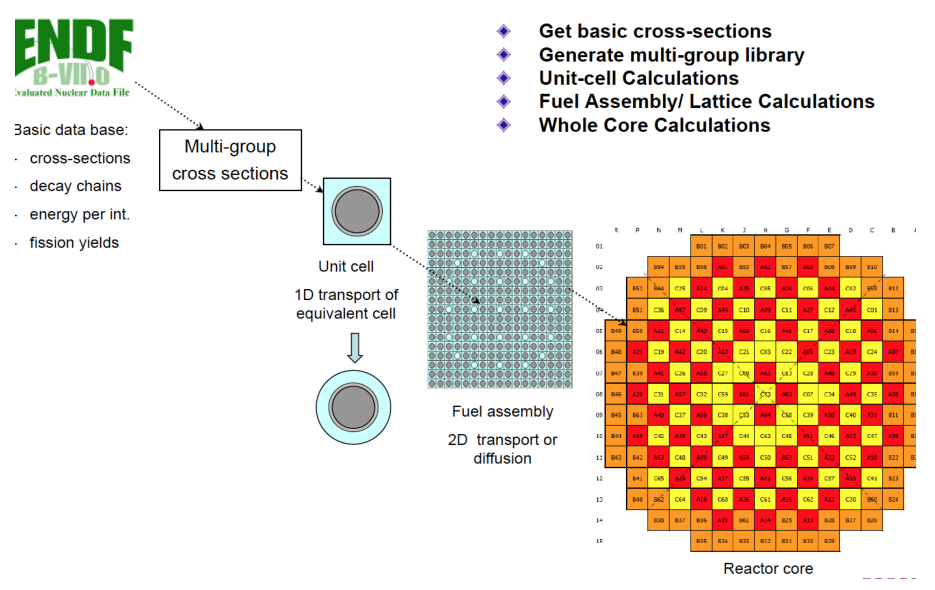
\includegraphics[width=6in]{images/design/lattice-nodal-code.png}
  \caption{Lattice Code Nodal Code Flowchart} \label{lattice-nodal-code}
\end{figure}


\clearpage
\subtopic{Lattice Code}
A lattice code calculation includes:
\begin{enumerate}
\item Pin spectrum calculation (energy domain, see Fig.~\ref{lattice-energy}). Lattice code solves for fine energy fluxes (1000s to 10,000s groups) with treatment of resolved resonances, and condense the cross sections to intermediate group cross sections (100s groups): 
  \eqn{ \sigma_{g} = \frac{\int_{E_{g-1}}^{E_{g}} \sigma(E) \phi(E) \dE  }{\int_{E_{g-1}}^{E_{g}} \phi(E) \dE}   }
\begin{figure}[ht]
  \centering
  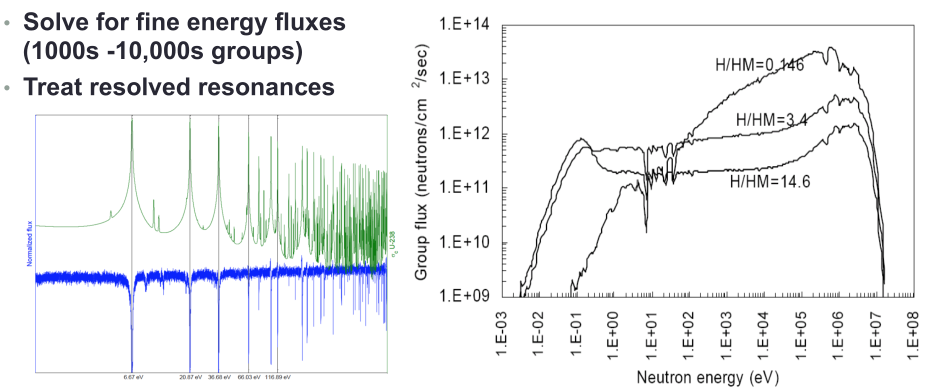
\includegraphics[width=4in]{images/design/lattice-energy.png}
  \caption{Lattice Code: Pin Spectrum Calculation} \label{lattice-energy}
\end{figure}

\item Intermediate group pin spatial calculation (spacial domain, see Fig.~\ref{lattice-space}). Lattice code solves for radial distributions of nuclides and fluxes in each type of pin. For a lattice depletion code, we want to know is the pin-wise isotropic inventories vs. BU. Lattice code produces data library as a function of fuel BU, coolant density, fuel temperature, void, etc (so lattice code does not just solve for a steady state condition, it solves for about 2000 cases). 
\begin{figure}[ht]
  \centering
  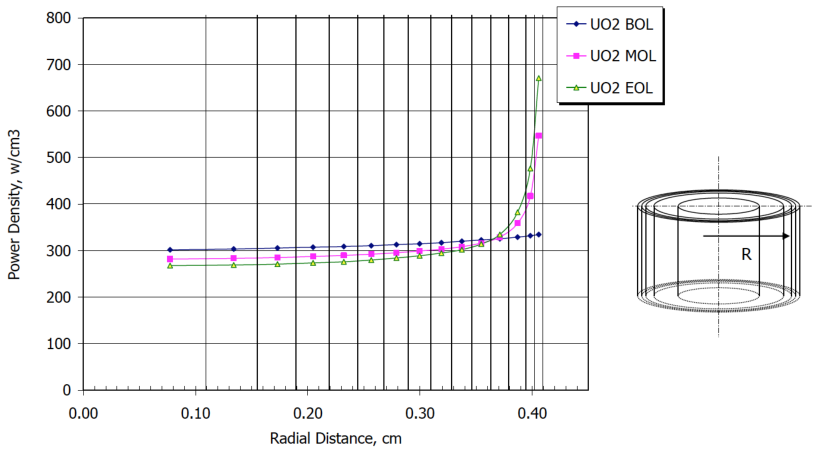
\includegraphics[width=4in]{images/design/lattice-space.png}
  \caption{Lattice Code: Pin Spatial Calculation} \label{lattice-space}
\end{figure}

\item Solve full assembly neutronics. Lattice code solves for pin-wise distribution of neutron fluxes (10-100 energy groups, homogenized pins). That's about 5000 spatial regions per assembly; MOC would take about 20 energy groups, 1000 angles, 0.05cm ray spacing. Then we compute $\keff$. 
\end{enumerate}

Comments: 
\begin{itemize}
\item One example of how lattice codes generate many lattices for possible uses: in PWRs, $\rho$ vs. BU (with no burnable poisons) are just straight lines depending on enrichment as in Fig.~\ref{lattice-rho-vs-BU}. Thus to achieve desirable long cycle and high BU, we need high enrichment, which is why almost all US fuel is around the 4-5\% enrichment level (currently fuels are made at 4.4\% enrichment; US regulation requires less than 5.2\% for trasportation reason).  
\begin{figure}[ht]
  \centering
  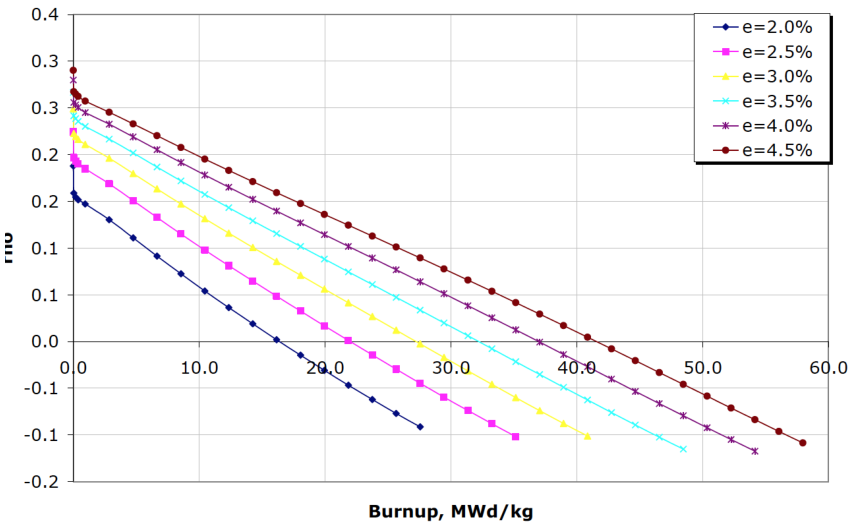
\includegraphics[width=4in]{images/design/lattice-rho-vs-BU.png}
  \caption{Lattice Code: PWR Assembly Reactivity vs. Burnup, Enrichment} \label{lattice-rho-vs-BU}
\end{figure}
\item Corner pin power peaking in PWRs: about 15\%.
\item Fission products absorption reduces reactivity of the fuel. 
\item U235 depletion significantly reduces reactivity as fissile inventory is reduced. 
\item Transmutation (particularly of U238) leads to complicated isotopic inventory. 
\item Pu239 production offsets part of the U235 reactivity depletion effects. 
\end{itemize}


\subtopic{Nodal Code}
A quick review of 3D advanced nodal codes: 
\begin{itemize}
\item 2D lattice transport/depletion calculation with approximated boundary conditions. 
\item 3D simulation using few group diffusion models with homogenization/condensation approximations. 
\item Fuel depletion on node-averaged basis: smooth intra-nodal spatial depletion representation. 
\item Local detail by superposition-based reconstruction. 
\item Pin conduction/bundle hydraulics: one characteristic pin and channel per bundle, no fluid cross flow between parallel channels, correlation-based heat transfer and void fraction models. 
\end{itemize}
Know the basic idea of the Transverse-integrate method: we transverse integrate 1D diffusion equation for the thermal group, approximate the source with 4th order Legendre polynomial, and solves for an analytical solution for the thermal group. Then we differentiate to get the net current at the interface, and use continuity of net currents/flux to get analytic expression for coupling. 




\clearpage
\topic{Uncertainty Analysis: Measurements}
We have a number of ways to determine the accuracy/uncertainty of core physics methods,
\begin{enumerate}
\item In-core flux mapping system: 58 instrumented locations and 61 (or 610) axial point measurements (through 58 tubes coming in from the bottom of the vessel). 
  \begin{itemize}
    \item Measurement should agree with simulation at core loading time to assure proper core loading. 
    \item Measurements will be performed monthly afterwards to assure compliance of power distribution with technical specifications (LHGR): verify peak LHGR with tech spec limits, verify pin/assembly burnup limits, determine 95/95 reliability factors for predictive models. 
    \item Zr spacers depress the flux because it displaces some water/moderator. 
    \item CMS codes provide very accurate power distribution, $\pm 300$pcm HFP core reactivity with depletion, and about 300pcm bias from CFP to HFP reactivity (Doppler, MTC) as see in Table~\ref{CMS-accuracy}. Notice TIP stands for Traversing In-core Probes, which are sensors inserted in the calibration tube of the LPRM assemblies to perform periodic calibration. Instrument tubes bend easily in BWRs, so BWRs tend to sample gamma for a more even distribution. 
      \begin{table}[ht]
        \centering
        \includegraphics[width=4in]{images/design/CMS-accuracy.png}
        \caption{BWR Predictive Accuracy of Nodal Codes} \label{CMS-accuracy}
      \end{table}
  \end{itemize}

\item Ex-core detector: calibrate based on flux maps, used to monitor core flux (power level) and axial power shape. 

\item HZP rod worth measurements. We solve IKE (given power extracted from the ex-core detector, we can back out $\rho (t)$ etc). Though when we are moving the rods, we cannot believe the point kinetics. That's why to perform a HZP rod worth measurement we have to wait: after a boron dilution, we move the rod in small number of steps, then wait. This takes more than 1 hours/rod, that's why dynamic rod worth calculation gets popular. Control rod worth has to be within 10\%.

\item Dynamic rod worth:  you pull rod out a little bit, then you drive your rod all the way in called banking (takes 2 minutes), then you pull the rod out again.  A subtle point here is that the power does not start to go up until the control rod is back in its criticality position (the power actually goes up a bit faster because of the delayed neutrons). Caution: flux should be high enough that statistics is reliable, but cannot be too high that the reactor goes critical.  See Section~\ref{dynamic-rod-worth} for more details. 
\end{enumerate}
Side note: Westinghouse designs have 228 notches in a control rod, CE has 100 notches. 



%%%%%%%%%%%%%% 10/04/12 22.39 Neutronics Lecture 2 %%%%%%%%%%%%
\clearpage
\topic{PWR Core Designs}
\subtopic{Reactivity Effects} 
We consider some common reactivity effects (negative effects): 
\begin{enumerate}
\item CZP $\to$ HZP: moderator temperature coefficients must satisfy limits.
  \begin{itemize}
  \item Moderator temperature coefficient cannot be too high; that is, boron concentration cannot be to high. Reason: when boron is high, adding more boron decreases the moderator density and increases the power. Sidenote: PWRs not only have boron in the coolant, but also in the rods.
  \item Moderator temperature coefficient cannot be too low (otherwise steamlines may break: the huge amount of secondary loop flow would remove all the heat out of the primary loop); that is, we need to be careful when we increase power/burnup, because the following terms contribute to a more negative moderator temperature coefficient: Doppler feedback, Xe build-up, balance out the change brought by Boron. 
  \end{itemize}
  \begin{figure}[ht]
    \centering
    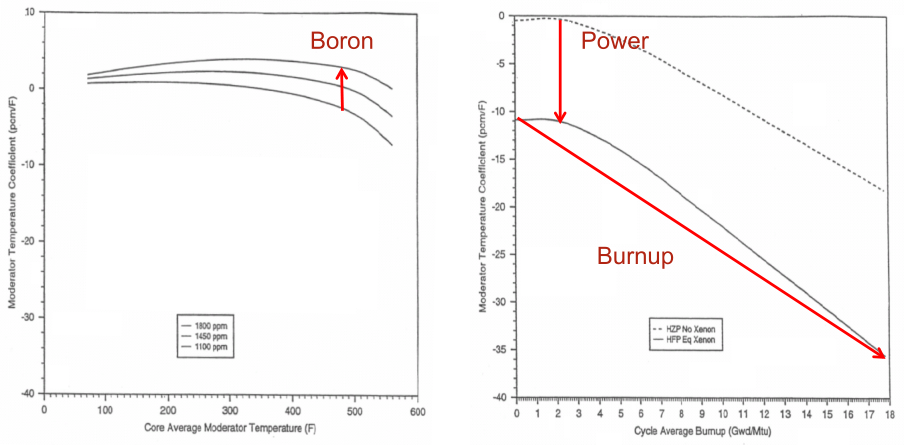
\includegraphics[width=6.5in]{images/design/moderator-temp-coeff.png}
    \caption{PWR Reactivity Effects: Moderator Temperature Coefficients} \label{PWR-rho}
  \end{figure}

\item \hi{HZP to HFP: $\rho \down$ due to resonance absorption (characterized by Doppler coefficient of reactivity).} As temperature increases, the thermal motion of the nuclei increases, causing a broadening of the cross section resonances and a lowering of their peaks. Because of the self-shielding of the nuclei in a material, the effective reaction rate $\up$ as temperature $\up$. Common isotopes that have large near thermal resonances: Xe135, Gd. 

\item \hi{During HFP: Xe and Sm build-up decreases $\rho$.} Recall Fig.~\ref{major-capture}, where Xe and Sm are most important when it comes to poisoning effect. We arrive at the following conclusions for the equilibrium concentration: 
  \eqn{ \left\{ \begin{array}{cc} I_{\infty} \propto \phi_0 & \phi_0 \up, I_{\infty} \up \\ X_{\infty} = \frac{(\gamma_I + \gamma_X) \Sigma_f \phi_0}{\lambda_X + \sigma_a^X \phi_0} & \phi_0 \up, X_{\infty} \mbox{ saturates.}   \end{array} \right. }

  Important concepts about Iodine/Xe:
  \begin{itemize}
  \item After startup, it takes about 30 hours for the two isotopes to reach saturation. 
  \item After shutdown, Xe peaks in 9 hours (because Iodine decays into Xe, adding about 3000 pcm reactivity) and decays away in 60 hours. 
  \item If we perform a rapid startup after a scram, Xe would be too high, thus the flux may be too high, which immediately burn out Xe and causing an \textbf{overshoot}. 
  \item Long term, a PWR core burns about 1000 pcm/month. So the 3000 pcm Xenon peak takes about 3 months to burn out. 
  \end{itemize}

  Important concepts about Pm/Sm: 
  \begin{itemize}
  \item After startup, it takes about 600 hours for the two isotopes to reach saturation. 
  \item After shutdown, Sm peaks in 200 hours, but never decay away unlike Xe. 
  \item Following a refueling outage, Sm reactivity peaks by 200-300 pcm after shutdown, and then return to equilibrium about 100 hours after restart. 
  \end{itemize}
  See Section~\ref{FP-Xenon} and \ref{FP-Sm} for more details.

\item \hi{HFP Xe equilibrium: fuel depletion decreases $\rho$.}
\end{enumerate}

\begin{table}[ht]
  \centering
  \begin{tabular}{c|c|c} \hline
    Condition & Reactivity effects & Decrease in $\Delta \rho$ \\ \hline
    CZP to HZP & Moderator density change & 2-5\% \\ \hline
    HZP to HFP & Resonance Absorption/Doppler Coefficient & 1-2\% \\ \hline
    \multirow{2}{*}{HFP, no Xe to Eq. Xe} & 0 to equil. Xe & 2-3\% \\ 
    & 0 to equil. Sm & 0.6\% \\ \hline
    HFP with Eq. Xe & Fuel depletion & 5-10\% \\ \hline \hline
    Total during startup &   & 4600-10,000 pcm \\ \hline
  \end{tabular}
  \caption{Summary of PWR Reactivity Effects} \label{PWR-reactivity}
\end{table}

\clearpage
\subtopic{Lattice Designs}
Step 1 of PWR core design includes picking the enrichment, number of assemblies, and cycle length. As illustrated in Fig.~\ref{areva-lattice-design}, if we pick 330 days as cycle length, then we need about 4\% enrichment and a reload fraction of 1/4.02. Take-away message: \hi{the average number of U235 is kind of conserved in the sense that enrichment $\up$, number of assembly $\down$} (which is good because less disposal cost). 

  \begin{figure}[ht]
    \centering
    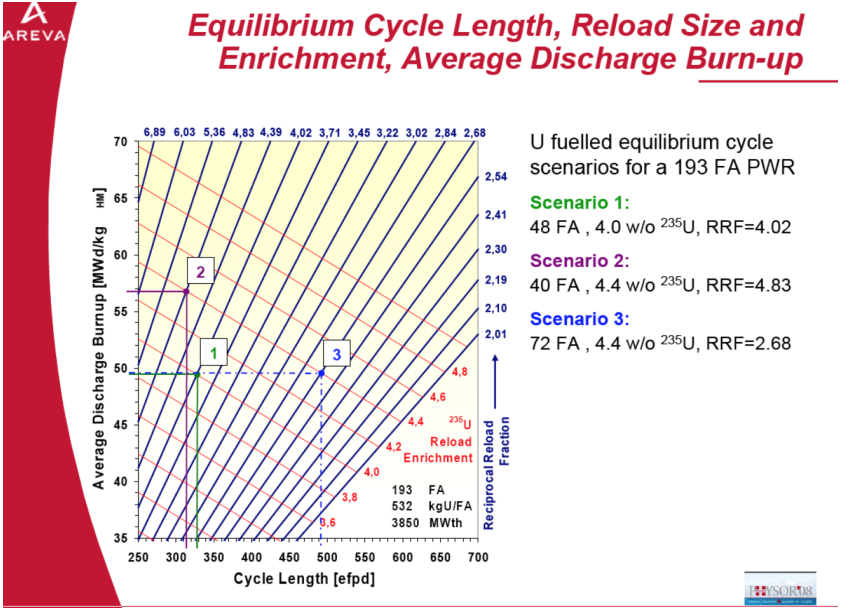
\includegraphics[width=4in]{images/design/areva-lattice-design.png}
    \caption{Areva's Chart Of Cycle length, \# Assemblies, Enrichment for PWRs} \label{areva-lattice-design}
  \end{figure}


\subtopic{Core Loading Patterns}
Step 2 of PWR core design is to pick a core loading pattern. One example is in Fig.~\ref{PWR-core-loading}, where it is important to surround new fuel with burned fuel to reduce local peaking, as we know fresh fuels can have a $\keff = 1.3$. 

\begin{figure}[ht]
  \centering
  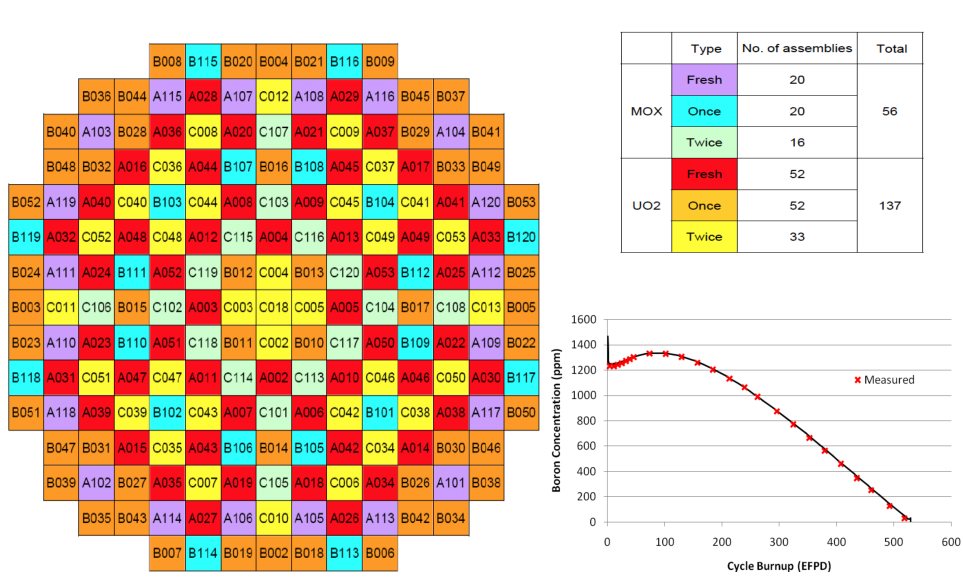
\includegraphics[width=4in]{images/design/PWR-core-loading.png}
  \caption{Sample PWRs Core Loading Pattern} \label{PWR-core-loading}
\end{figure}

We consider two famous patterns: 
\begin{enumerate}
\item Out/In Pattern. Notice the depletion terminates when boron becomes zero. Also the power peaking factor as a function of time increases first and then decreases. 
\begin{figure}[ht]
  \centering
  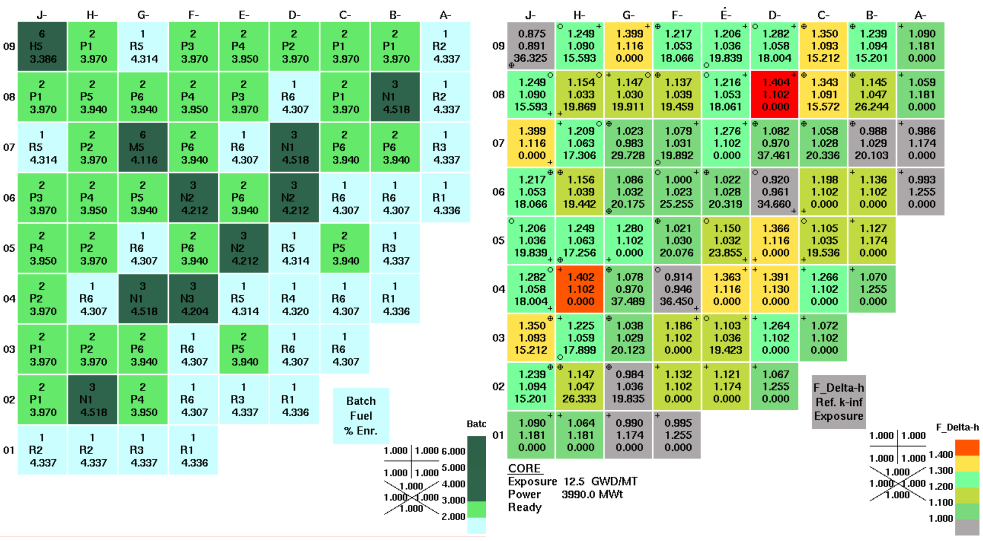
\includegraphics[width=5in]{images/design/PWR-out-in.png}
  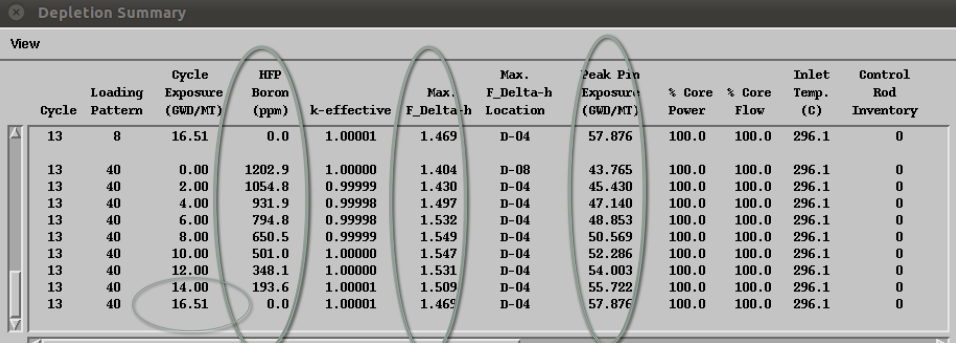
\includegraphics[width=5in]{images/design/PWR-out-in-2.png}
  \caption{PWR Out/In Loading Pattern} \label{PWR-out-in}
\end{figure}

\item In/In/Out Pattern (low leakage): the center fuel is taken from ancient batch; new fuels are surrounded by burned fuel; power at periphery is reduced. 
\begin{figure}[ht]
  \centering
  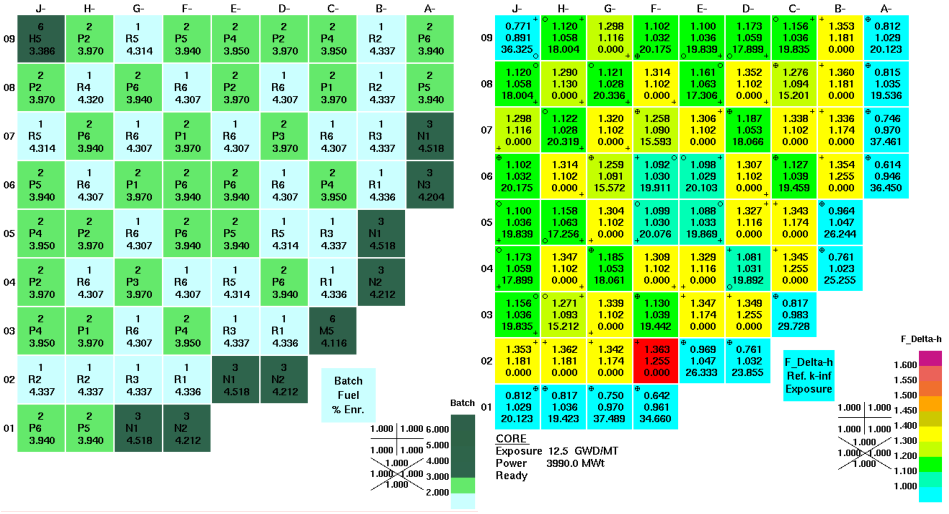
\includegraphics[width=5in]{images/design/PWR-in-in-out.png}
  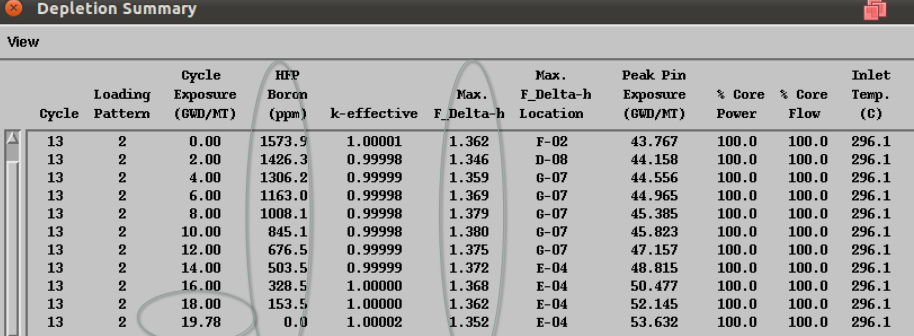
\includegraphics[width=5in]{images/design/PWR-in-in-out-2.png}
  \caption{PWR In/In/Out Loading Pattern} \label{PWR-in-in-out}
\end{figure}
\end{enumerate}


\subtopic{PWR Reactivity Control} 
In PWRs, about 1/2 assemblies have no control rods, so we need to use burnable absorbers etc. 
\begin{enumerate}
\item Burnable absorber. To control reactivity/power peaking in the In/In/Out pattern, we place burnable absorber (30,000pcm) in the interior fresh assemblies, and place no burnable absorber in the exterior assemblies (without burnable absorber, the power may be peaking by a factor of 3). 

\item IFBA: pro is that it can be placed anywhere as it is just a thin layer of coating outside of fuel pins. The drawback is that IFBA produces He, which pressurizes the fuel pin and thus we need to design the core with extra platinum space or to use empty blanket. 
\end{enumerate}


\subtopic{Cycle Length and Equilibrium Cycle}
We want to cluster fresh fuels (which is a good thing for $\keff$), but could lead to bad power peaking. To estimate cycle length though, we can place ALL fresh fuels on the inside and the depleted on the outside for a pretty accurate estimate of cycle length. 

An important fact is (know how to calculate the following for the qual), 
\eqn{ \boxed{ \mbox{1 Gwd/MT} = 30 \mbox{ days} = 30 \mbox{ million dollars} } }

Equilibrium cycle: we repeat the same core shuffle pattern cycle after cycle until the cycle length stops changing as in Fig.~\ref{PWR-equil-cycle}. Desirable features we are looking for: very flat peak power, and power peaks moves from assembly to assembly between cycles. In practice, it is also common to design a 2-3 cycle pattern and repeat the pattern until equilibrium.
\begin{figure}[ht]
  \centering
  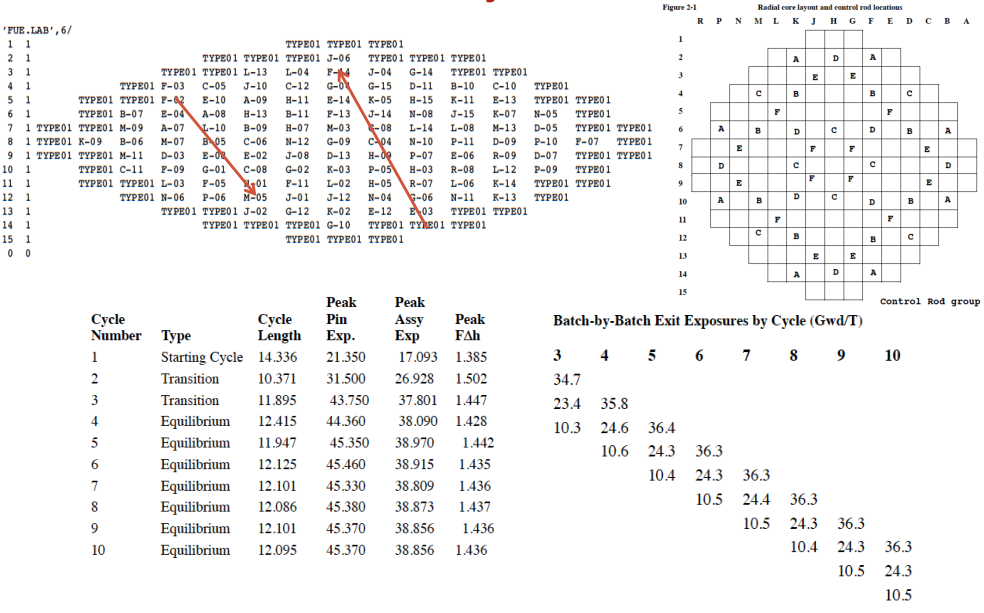
\includegraphics[width=5in]{images/design/PWR-equil-cycle.png}
  \caption{PWR Equilibrium Cycle} \label{PWR-equil-cycle}
\end{figure}


\clearpage
\topic{BWR Core Designs} 
Now we move to BWR core designs. A major difference is that BWRs are bigger than PWRs and thus reducing the power density from PWRs' 100 kW/L to BWRs' 50 kW/L. Reference: \href{http://www.ne.doe.gov/np2010/pdfs/ABWRReactorCoreNeutronics.pdf}{GE's ABWR seminar by LE Fennern}.

\subtopic{Design Criteria} 
Table~\ref{BWRs-criteria} lists the most important reactor physics core design criteria translated into plant technical specifications.
\begin{table}[ht]
  \begin{tabular}{|l|l|l|} \hline
    Condition & Criteria & Abbreviation \\ \hline
    \multirow{3}{*}{Pseudo Steady State} & Shut down margin (cold, highest worth rod out)  & SDM \\ 
    & Max notch worth for startups &  \\
    & Max linear heat generate rate & MLHGR \\ \hline
    Normal Operations & Min critical power ratio & MCPR \\ \hline
    LOCA Limits & Max average planer heat generation rate & MAPHGR \\ \hline
    RIA Limits & Max calories per g enthalpy limit & CPG \\ \hline
  \end{tabular}
  \caption{BWRs Design Criteria and Acceptance Criteria} \label{BWRs-criteria}
\end{table}
For instance, 
\begin{itemize}
\item LOCA limit describes local behavior which is related to local power generated. 
\item CPR is sensitive to spacers (because of dryout condition). When power increases or flow decreases, CPR tells us what thermal margin we have. 
\item MCPR is chosen from generic transient analysis. Core design is performed to satisfy those limits. 
\item Linear heat generation rate limits.
  \begin{figure}[ht]
    \centering
    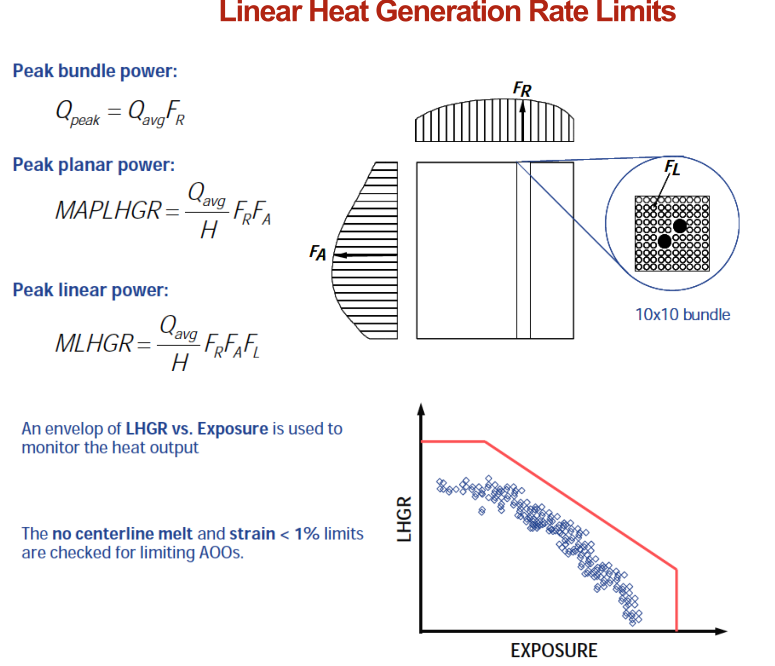
\includegraphics[width=4in]{images/design/BWR-LHGR.png}
    \caption{Linear Heat Generation Rate Limits} 
  \end{figure}
\item MAPLHGR tech spec are designed to cover LOCA (eg., peak cladding temperature). 
  \begin{figure}[ht]
    \centering
    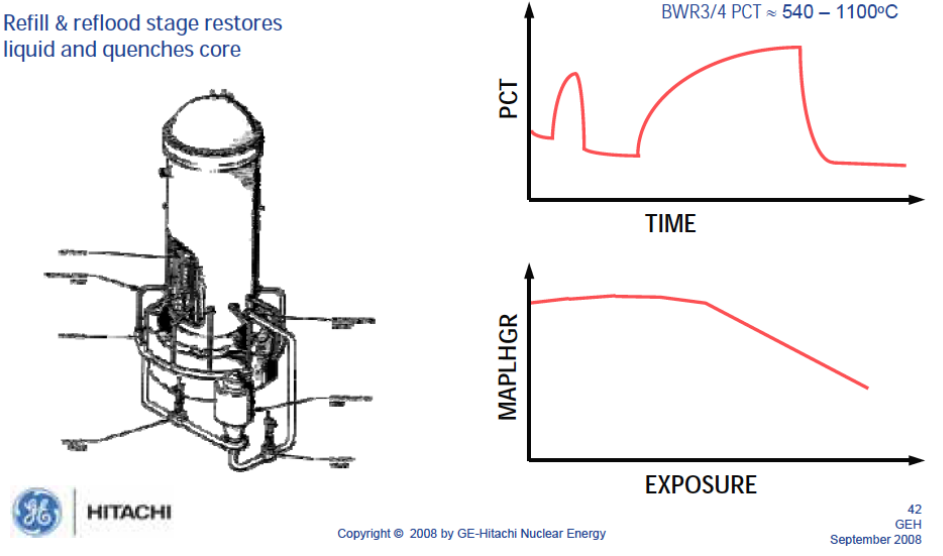
\includegraphics[width=4in]{images/design/BWR-MAPLHGR.png}
    \caption{MAPLHGR Designed to Cover LOCA} 
    \end{figure}
\end{itemize}



\subtopic{Core Designs}
Overall BWR core designs (lattice designs, core loading patterns) are nightmares because: BWRs have 800 assemblies compare with PWRs' 193; BWRs runs with CR inserted, while PWRs do not run with CR inserted; BWRs have no soluble boron (because we do not want to boil boron everywhere) thus we have to rely on other control mechanism. 
\begin{enumerate}
\item Modern trend has been pushing the fuel limits (increasing the power density from 40 kW/L to 50 kW/L to even higher as seen in Fig.~\ref{BWR-fuel-limits}. The issue with higher power density is that we need to install bigger pumps and deal with more vibration issues. 
  \begin{figure}[ht]
    \centering
    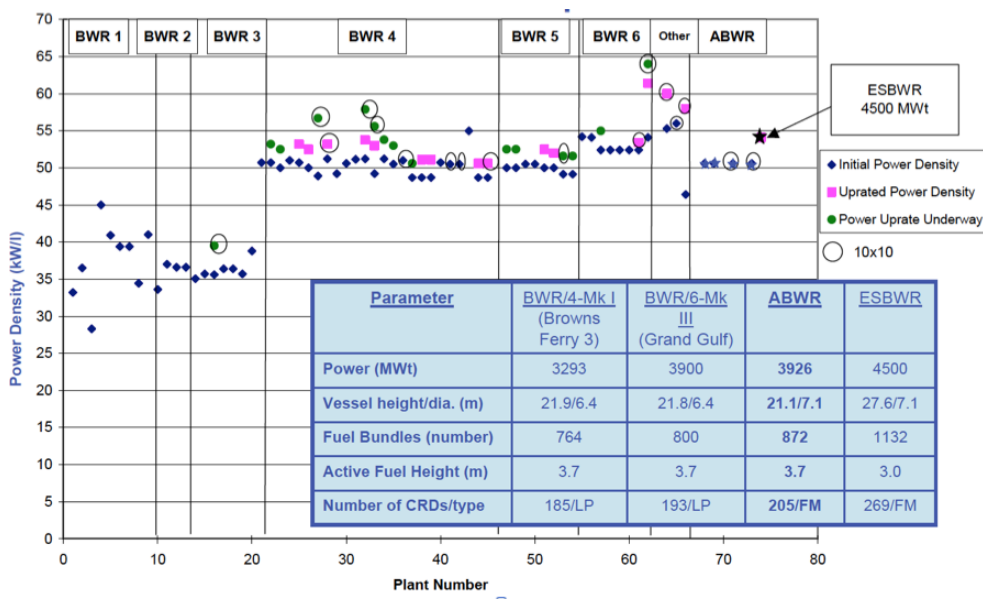
\includegraphics[width=4in]{images/design/BWR-fuel-limits.png}
    \caption{BWR Fuel Limits} \label{BWR-fuel-limits} 
    \end{figure}

\item Also 7x7 bundle are being pushed towards 11x11 bundle, which means linear heat generation rate decrease, though CPR may or may not increase. 

\item Simple Control Cell Core (CCC) has been used by many annual cycles (common in Europe). The motivation is, when CRs are pulled out, local peaking factor would increase, thus a CCC with 20\% fresh fuel and low BU would be easy for an annual cycle. Though this is not the case in the US as there are not enough locations for CCC because we need to put about 37\% fresh fuel to sustain a longer cycle length. Again in CCC notice the check board pattern in which fresh fuels are surrounded by depleted fuel. 
  \begin{figure}[ht]
    \centering
    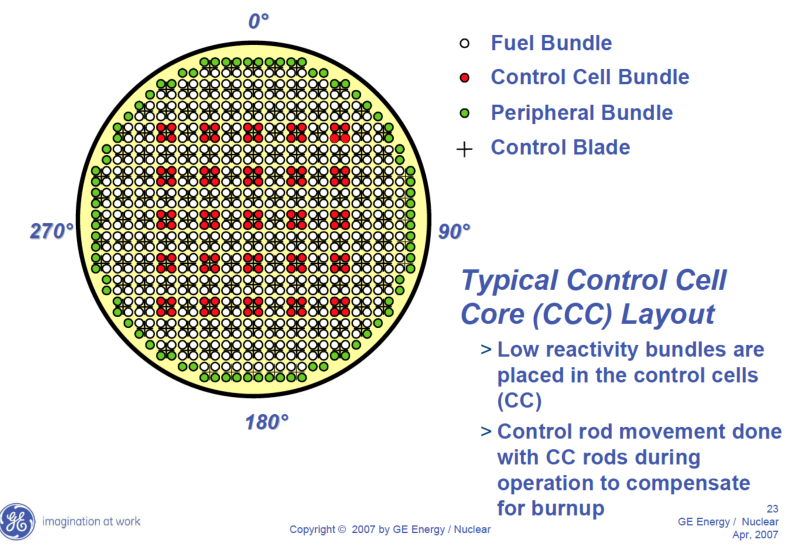
\includegraphics[width=4in]{images/design/BWR-CCC.png}
    \caption{BWR Control Cell Core (CCC) Layout} \label{BWR-CCC} 
    \end{figure}
\end{enumerate}



\subtopic{Operational Analysis, Reactivity Control}
Keep in mind that BWRs can operate at various flow rate (unlike PWRs whose flow rate is fixed).  There are three modes we consider for BWRs (to extend cycle length): 
\begin{enumerate}
\item Spectrum shifted operation: operate at reduced flow (70\%) to increase void, thus decreasing fuel density, hardening the spectrum, increasing U238 resonance absorption and produce more Pu, which would extend the cycle length. 
\item Increase core flow operation.
\item Coast down: maximize flow to increase reactivity, thus lowering feed water temperature and the power would coast. Coast down can last as long as 3 months down to 50\% power. 
\end{enumerate}
  \begin{figure}[ht]
    \centering
    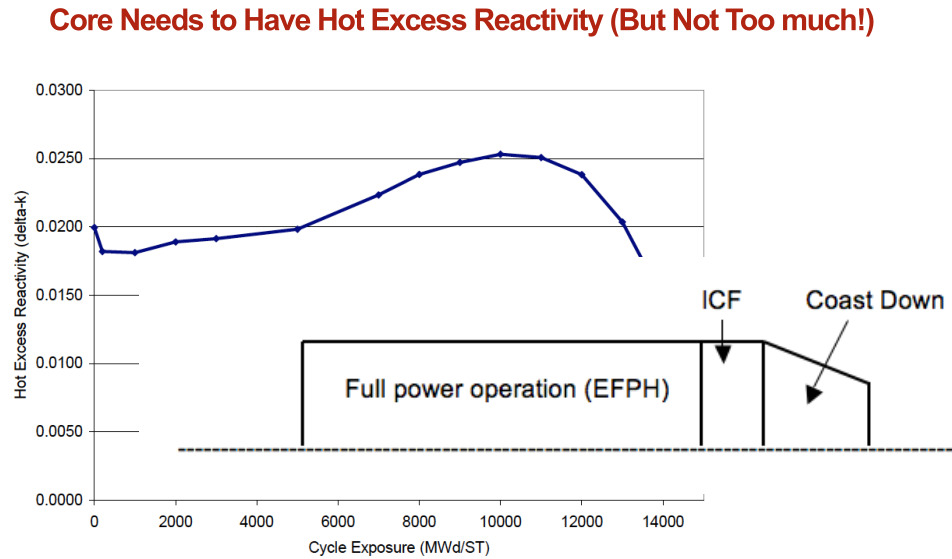
\includegraphics[width=4in]{images/design/BWR-excess-rho.png}
    \caption{BWRs Need to Have Hot Excess Reactivity} \label{BWR-excess-rho} 
    \end{figure}

There is a need to have hot excess reactivity, though we want to keep the reactivity swing flatter. Eg., \hi{PWRs have 20\% $\Delta k$ reactivity hold-down, whereas BWRs only have 2\% $\Delta k$ (the additional comes from Gd)}. Gd is integrated with fuel, very self-shielding with huge $\Sigma_a$, and behave like onion skin burning\footnote{Onion skin burning is used to describe when the cross section is very large ($\sigma_{Gd} = 10^6$b), a thin layer of the material would be burned out, then another thin layer slightly inside would be burned out, etc, like an onion peeling}. So the advantage of Gd over IFBA is the Gd can control burning by density as in Fig.~\ref{BWR-Gd} whereas IFBA can only burn constantly. We pick the Gd concentration and number of pins to flatten the reactivity vs. BU plot. Notice in Fig.~\ref{BWR-Gd}, 
\begin{itemize}
\item Know how to extrapolate to get no-Gd curve thus the hold-down. 
\item 10 times Gd concentration only produces 25\% more hold-down due to self-shielding. 
\item If put in enough Gd, the curve could be totally flat. 
\item In one bundle, we can put multiple concentration of Gd. For instance, Sweden has done pellet-by-pellet design where every other pellet is all Gd. 
\end{itemize}
  \begin{figure}[ht]
    \centering
    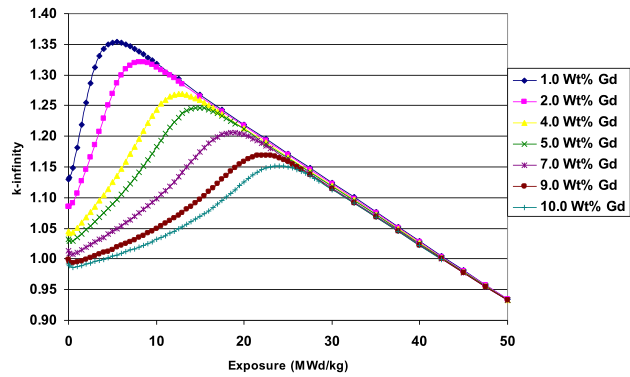
\includegraphics[width=4in]{images/design/BWR-Gd.png}
    \caption{BWRs Reactivity Flattening using Gd} \label{BWR-Gd} 
    \end{figure}

BWRs generate high void at top of the core which means that the bottom fuel is more burned, there are more fuel left on the top, and the flow is reduced at the top. To compensate for the bottom-heavy flux, we consider: 
\begin{enumerate}
\item Add water rods to keep more coolant in the top. 
\item Add part length fuel rods to allow for more water at the top. 
\item Have more absorber rods in the bottom of the bundle. 
\item Use axial enrichment zoning to flatten the power. 
\item Insert some shallow rods in the bottom of the core. 
\end{enumerate}

Comments:
\begin{enumerate}
\item PLRs make lattice more over-moderated when cold and lower reactivity (which is a shutdown margin improvement). 
\item Deep inserted CR controls reactivity; shallowly inserted CR controls power peaking. 
\item Towards the end of the cycle, we slowly remove all CRs, suddenly all the power rolls to the top, in which case we can lose all CPR margin. Thus end-of-cycle condition can be more limiting for BWRs as in Fig.~\ref{BWR-end}. 
  \begin{figure}[ht]
    \centering
    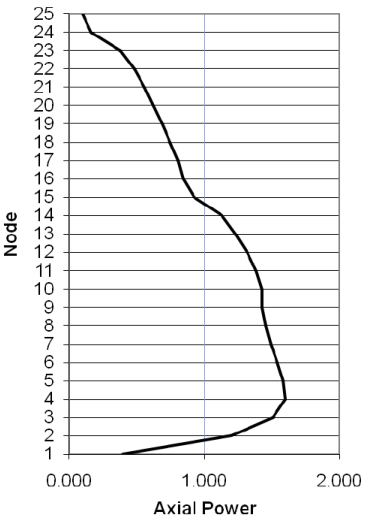
\includegraphics[width=2in]{images/design/BWR-BOC.png}
    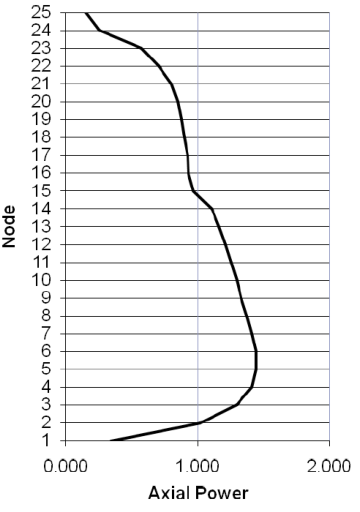
\includegraphics[width=2in]{images/design/BWR-MOC.png}
    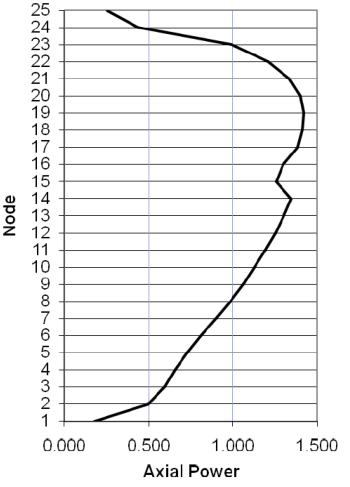
\includegraphics[width=2in]{images/design/BWR-EOC.png}
    \caption{BWRs Axial Power Shapes at BOC, MOC, and EOC} \label{BWR-cycle} 
    \end{figure}



  \begin{figure}[ht]
    \centering
    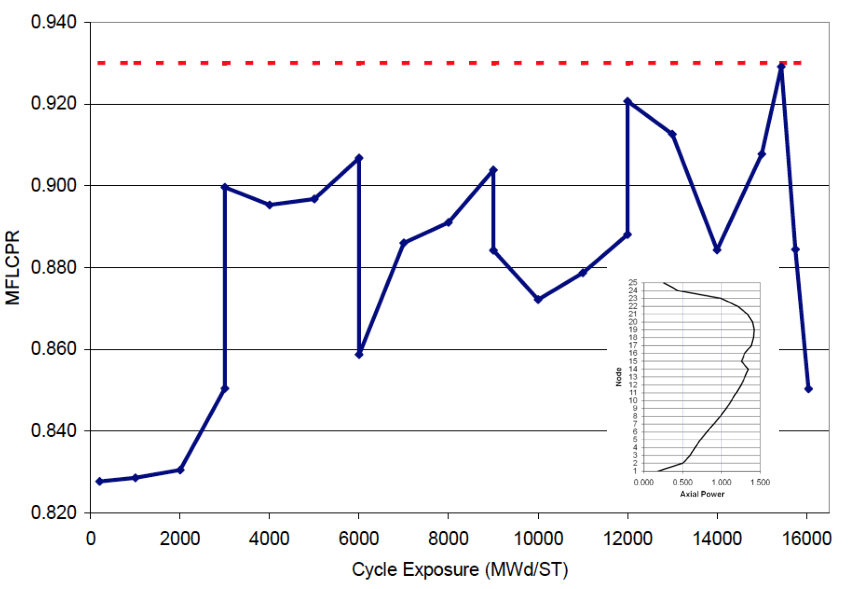
\includegraphics[width=4in]{images/design/BWR-limiting-end.png}
    \caption{BWRs MFLCPR More Limiting Near End of Cycle} \label{BWR-end} 
    \end{figure}
\end{enumerate}



The last step is illustrated in Fig.~\ref{BWR-startup}, as we design the startup sequence (power, flow and rods) when the core design is finished.
  \begin{figure}[ht]
    \centering
    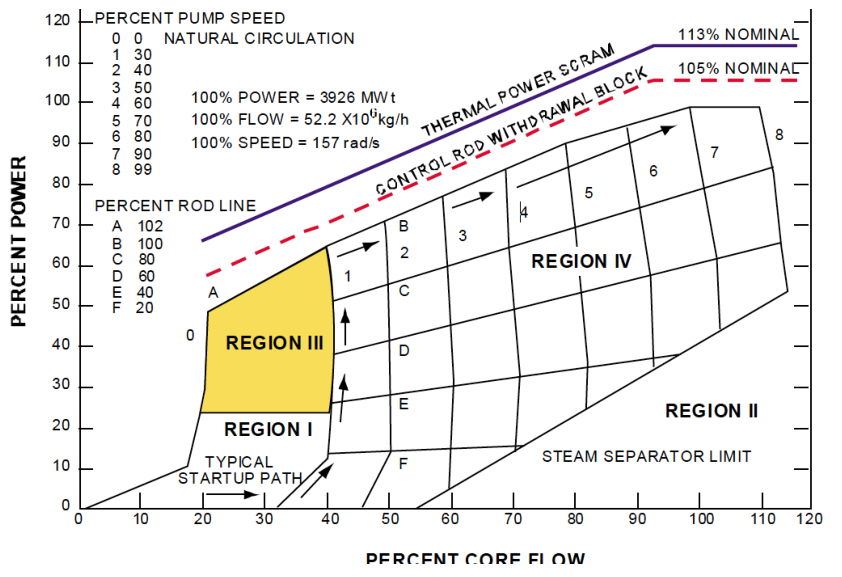
\includegraphics[width=6in]{images/design/BWR-startup-seq.png}
    \caption{BWRs Design for Startup Sequence} \label{BWR-startup} 
    \end{figure}


\clearpage
\topic{PWR Core Loading Pattern Optimization} 

Reference: Turinsky's `Core Isotopic Depletion and Fuel Management' in
\textit{Handbook of Nuclear Engineering}, Springer (2010). Objectives: 
\begin{itemize}
\item Limit on power peaking. 
\item Increased margins to thermal limits (CHF, T$_{\mathrm{fuel}}$). 
\item Maximize economics. 
\end{itemize}


\subtopic{Fundamentals}

The \textbf{fundamental trade off} is between economics (maximize energy) and
minimize safety risks (minimize peaking):

\begin{itemize}
\item Maximize energy: maximize EOC reactivity, maximize cycle length,
  maximize fuel burnup.
\item Minimize peaking: minimize maximum enthalpy rise hot-channel
  factor F$_{\Delta H}$, minimize heat flux hot-channel factor.
\end{itemize}

\textbf{Common loading patterns}: 

\begin{enumerate}
\item Out-in: most burned fuel bundles are loaded on the
  inside. Result: reduced peaking factor (e.g., 1.404), but bad
  economy (for instance, when an outer ring fresh fuel bundle has a
  kinf of 1.25, and the whole core has a keff of 1, that implies that
  about 25\% of the neutrons leak out).

\item In-out: most burned on the outside. good peaking factor, bad economics.

\item Ring of fire (or low leakage pattern, in/in/out pattern):
  checker board pattern of fresh and one cycle fuel, with a ring of
  burned one near the out-side most. We get about 3 months additional
  operating time compared with the traditional out-in pattern.
\end{enumerate}

A note here is that a big difference between PWRs and BWRs is that: 

\begin{itemize}

\item PWRs: density is almost constant; a fuel shuffle affects the
  global problem and can produce flux tilting very easily.

\item BWRs: because of the existence of void, effects tend to be local. 

\end{itemize}


On a high level, a loading pattern problem

\begin{itemize}
\item is a nonlinear, mixed-integer problem (so no derivatives).
\item is inherently a multi-objective problem. 
\item is highly constrained. 
\item has disjoint feasible regions.
\item has an extremely large decision space. 
\end{itemize}



\clearpage

\subtopic{XIMAGE: Loading Pattern Design} 

\href{http://www.studsvik.com/Business-Areas/Operating-Efficiency/Nuclear-Fuel-Analysis-Software/Loading-Pattern-Design/XIMAGE/}{XIMAGE}
is basically a graphical tool that runs CASMO and SIMULATE underneath
and displays the results nicely for easy visualization. For this class
we use X-IMAGE to optimize PWR loading pattern (quarter core
shuffling). BWR loading pattern is more difficult because:

\begin{itemize}

\item BWRs typically do half core shuffling. There are four times as
  many bundles as in PWRs.

\item Multiple rod patterns are always possible, and rods must be
  moved for criticality.

\item Flow is a variable. It is common to drive pump speed to control
  reactivity (review load-follow). Because a harder spectrum is
  beneficial for extending cycle length, typically we want to run the
  core with a low flow rate for as long as we can, then slowly
  increasing the flow rate.
\end{itemize}


There are a couple of terms used in XIMAGE: 

\begin{enumerate}

\item \textbf{Boron search}: at each cycle exposure, a search is
  performed to find the Boron concentration that achieves a $\keff =
  1$.

\item \textbf{F-Delta h}: $F$ is the power peaking factor, and $\Delta h$ is
  the entropy increase. This is a good measurement because it takes
  into account that not all energy generated from fission would be
  deposited locally. For instance, gamma interactions in the
  structural material generate heat which is then picked up by the
  fluid and reflected in $\Delta h$. The analog in BWR is the MCPR
  (Minimum Critical Power Ratio).

\item \textbf{Equilibrium cycle calculation}: assume the shuffling
  pattern (called the equilibrium cycle) stays identical from cycle to
  cycle. The cycle length converges fairly quickly (e.g., in this case
  5 cycles for a PWR). Though in real life, the condition never stays
  perfectly identical from cycle to cycle, so small variation
  exists. Typically a year before start-up, someone designs the core
  loading pattern, and this design finalizes about 6 months before the
  actual start-up of the plant.
\end{enumerate}


Some help in using XIMAGE: 

\begin{itemize}

\item Right click gives option, middle click gives configurations (for
  instance, display maps -- left and right maps is a useful ting to
  do). Use `View-Map layout' option on the top menu to change
  displayed terms.

\item Shuffle: octant shuffle would touch four assemblies to keep the
  octant symmetry. There might be warning messages. For instance, PWR
  has odd number of assemblies along each side, so you cannot shuffle
  anyone on the axis.

\item Assembly inventory (automatically opened window). First box is
  fresh fuel, second box is depleted fuel, and third box contains
  depleted fuel that is

\item Click on a patter in the LP window, right click on the map to
  restore that pattern.

\item Middle click to bring up LP library to name the loading pattern. 

\item Rotate the exterior assemblies: circle means minimum exposure,
  typically you move them inwards. You typically look at the BOC Boron
  concentration to be high.

\item After finding a good pattern, do an equilibrium cycle search to
  see find the final equilibrium parameters.
\end{itemize}

For this class, we optimize for maximum cycle length, $F \Delta h <
1.60$, MTC $<$ 3 pcm/C. cycle length: 18.5 

\clearpage

\subtopic{Greedy Binary Random Swap in Quarter Core}

It takes XIMAGE about 2 seconds to perform a 24-axial-node cycle
depletion. That is about 14,400 patterns per workday. But the limiting
factor is on the human side that we have limited decision speed,
limited persistence, unable to recognize already searched space, and
we tend to be greedy. That is why we move to automated optimization
that avoids the above limitations. The simpliest method is to perform
a greedy binary random swap in quarter-core:

\todo[inline]{add in greedy binary random swap} 

\begin{algorithm}
  \begin{algorithmic}
    \STATE Intialize $x, C_0, L_0$.  $k=0$. 
    \WHILE{not converged} 
    \STATE do 
    \ENDWHILE
  \end{algorithmic}
  \caption{Basic Greedy Binary Random Swap Algorithm}
\end{algorithm}

The question is, how do we make search faster? 

There are a couple of issues we need to keep in mind: 

\begin{enumerate}

\item No removable BPs under control rods. 

\item Rods have to have limited burnup (say 30 MWd/kg) under control
  rod positions). The main reason is that guide tube distorts when
  burnup is high, and the control rods may not go in. The secondary
  reason is that we want the reasonable rod worth underneath the
  control rods.

\item We prefer quadrant/octant symmetry in the fresh fuel. Likely
  wise we can maintain batch symmetry in the depleted fuel.

\item Use heuristics to eliminate unattractive patterns: 
  \begin{itemize}
    \item No fresh fuel on periphery. 
    \item Template heuristics. 
  \end{itemize}

\item Use `surrogate model' to replace expansive function
  evaluation. In most optimization, it takes more time to decide the
  next step than to perform the function evaluation. For our problem,
  the function evaluation takes significantly longer than the decision
  for next step.
  \begin{itemize}
  \item Early stages we can use 2D rather than 3D.
  \item Early stages we can use neural network. 
  \item Don't complete cycle depletion if first state point is not
    acceptable. 
  \end{itemize}
\end{enumerate}





\clearpage
\subtopic{Stochastic Optimization Schemes}

\textbf{Casting the objectives}: A common way for using multiple objectives is
the \hi{augmented (weighted) objective}. Example for $k, p$: 

\eqn{ f(k,p) = (1.5 - p) - 100 H (1.15 - k) }

This is an easy way to include constrains as penalties. A better
approach would the Pareto optimal which is not covered in this lecture
(Ask stephano for questions).


Stochastic optimization schemes are only real options, 

\begin{enumerate}
\item \textbf{Simulated Annealing}: The physical process of annealing
  means bringing metals to a high temperature and let it cool slowly;
  if it cools slowly enough eventually it would get to its minimum
  energy.

\begin{algorithm}
  \begin{algorithmic}
    \STATE Intialize $x, C_0, L_0$.  $k=0$. 
    \WHILE{not converged} 
    \STATE do 
    \ENDWHILE
  \end{algorithmic}
  \caption{Basic Simulated Annealing Algorithm} 
\end{algorithm}

\item \textbf{Genetic Algorithm}
  \begin{algorithm}
    \begin{algorithmic}
      \STATE Create and evaluate an initial population of $N$ chromosomes.
      \WHILE{not converged} 
      \STATE Select $n$ chromosomes to reproduce (crossover); 
      \STATE Crossover and/or Mutate chromosomes;
      \STATE Replace $n$ least fit chromosomes with $n$ offsprings;
      \STATE Evaluate the population.
      \ENDWHILE
    \end{algorithmic}
    \caption{Basic Genetic Algorithm}
  \end{algorithm}

  \begin{enumerate}
  \item  Selection criteria: survival of the fittest. 
    \begin{enumerate}
    \item Proportional selection, Russian-Roulette. 
    \item Find the fittest one? 
    \end{enumerate}

  \item Crossover: breeding patterns. This type of problem is called
    ordering problems: we have finite number of something that need to
    be conserved in the crossover. A typically way to do it is the
    Heuristic Tie-Breaking crossover:

  \item Mutation: add a bit of local refinement to the global scopes of GA. 

  \item Replacement: 
    \begin{enumerate}
    \item Delete all (generational): replace all $N$ parents with $N$
      offspring.  

    \item Steady state: replace some subset of $n$ parents with or
      without avoiding duplication.
    \end{enumerate}
  \end{enumerate}


\item Swarm intelligence (ant colony, particle swarm, etc). 
\item Greedy Exhaustive Dual Binary Swaps (GEDBS). 
\end{enumerate}

\textbf{Comparison between SA and GA}: 

\begin{itemize}
\item SA is simpler to understand. SA is harder to parallelize (because
  at each temperature you are making up a $L$ that depends on the
  previous steps).

\item GA is natural for true `multiobjective' optimization. GA is
  trivial to parallelize.

\item Both are heuristic and need some tuning. Both can be improved
  with hill-climbing heuristics (eg, greedy exhaustive single binary
  swaps).
\end{itemize}

A subtle point: once you put the most burned cores on the outside-most
ring, how the inside pattern does not affect the cycle length anymore
because the power on the outside is so small. But the peaking power is
very sensitive on the inner pattern.



\clearpage
\end{document}
